\subsection{Vibration Testes}\label{ssec:vibrationTests}

	\subsubsection{Configuration and Background}

		As mentioned in Section \ref{sec:vibration-acquisition-channel}, the \textit{Vibration Acquisition Channel} can be seen as a protection circuit that allows a input signal from 0 to 3.3V inside a frequency bandwidth of 1.6kHz to pass to the microcontroller's analog to digial converter.
		\par
		In order to test this interface, a \textit{Full Stop Test} similar to the one from Section \ref{ssec:full-stop-test} was performed. However, with only 10 snubs and this time, only the rotor spinning frequency and the accelerometer signal were monitored. Moreover, the rotor spinning frequency was also monitored when the machine was stabilizing at the upper speed limit.

		Figure \ref{fig:test-vibration-assembly} shows how the vibration sensor was assembled, it was positioned in a way that the axis which the acceleration was going to be measured would be perpendicular to the rotational shaft.

		\begin{figure}[htbp]
			\centering
			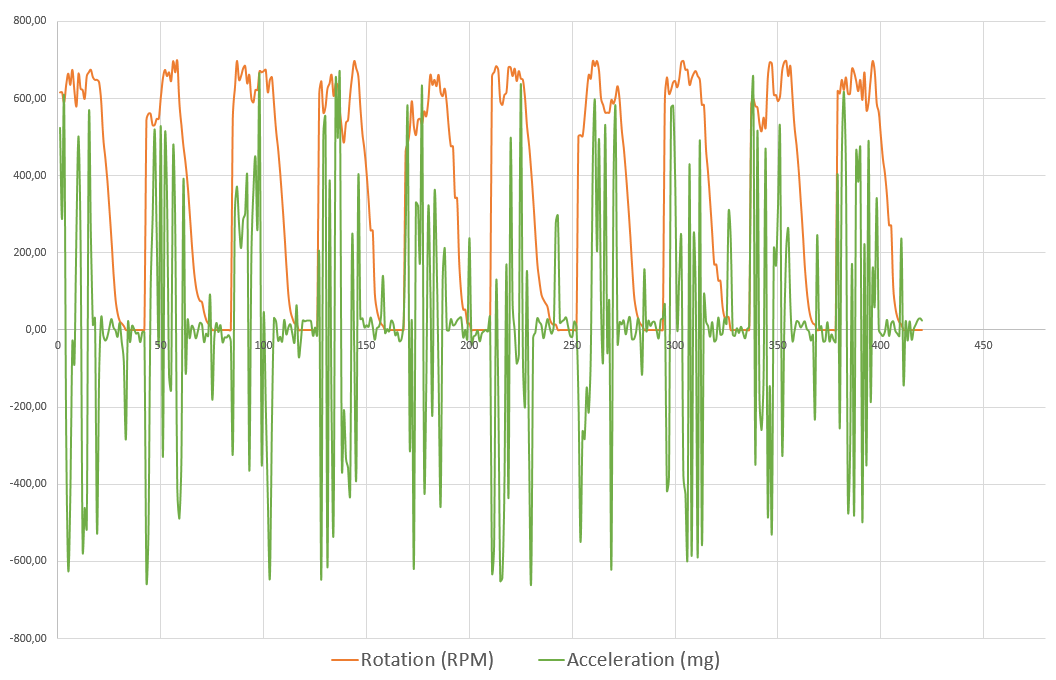
\includegraphics[width=.9\textwidth]{figuras/fig-test-vibration-assembly}
			\caption{Vibration Sensor Positioning}
			\label{fig:test-vibration-assembly}
		\end{figure}

	\subsection{Results}	

		Figure \ref{fig:test-vibration} shows the results from the vibration test, each of the orange pikes represent a snub. Moreover, it is important to state that \textit{mg} means $10^-3 \cdot 9.8 \frac{m}{s^2}$ and not miligrams.

		\begin{figure}[htbp]
			\centering
			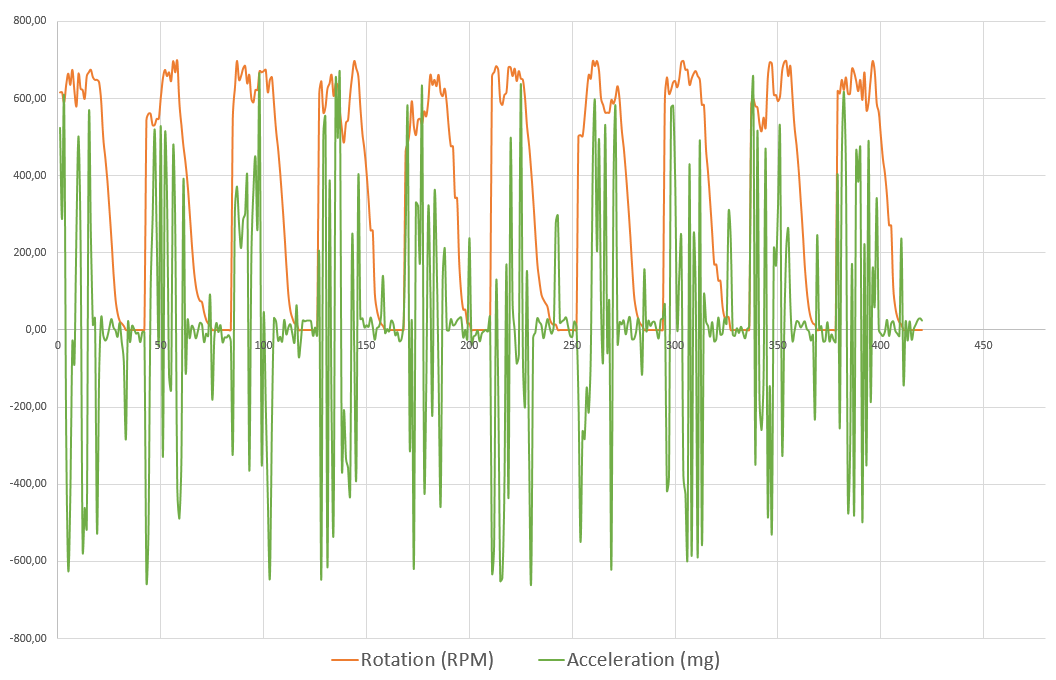
\includegraphics[width=.9\textwidth]{figuras/fig-test-vibration}
			\caption{Vibration Acquisition Channel Test Results}
			\label{fig:test-vibration}
		\end{figure}

	\subsubsection{Discussion}

		The goal of this tests was to show how the acceleration perpendicular to the shaft would vary along a testing snub. From the results it is possible to take the following conclusions:

		\begin{itemize}
			\item The acceleration, \textit{i.e.} vibration of the machine is greater when the rotor is spinning. The average acceleration during this phase was 336.73 mg.
			\item At each snub, when the brake phase starts, \textit{i.e.} when the rotation starts to decrease, vibration is minimal, almost none, probably noise has a great contribuition to this signal. The average acceleration during the braking phase was 23.67 mg.
			\item During the act of release of the brakes, when the rotor reach the lower speed limit, there is a small peak of vibration.
			\item When the brake is released and the motor is turned off, the vibration is quite small. The average acceleration during the this phase was 40.80 mg.
		\end{itemize}

		It was also clearly that the vibration range of the choosen sensor,-3g/+3g \cite{devices2010adxl335} was too wide for the measurements, the absolute maximum measured acceleration value was 656 mg (or 0.652g). A sensor with a narrow measurement range would better suit this application.